\documentclass{beamer}
\usetheme{default}
\usepackage{hyperref}
\usepackage{bookmark}
\usepackage{graphicx}
\usepackage{amsmath}    % for advanced math
%\usepackage[margin=1in]{geometry} % Adjust margins as you like
\usepackage{amssymb}    % for additional math symbols
\usepackage{setspace}
\usepackage{cite} 

\onehalfspacing

% Title, author, and date
\title[Turbulent Flow Project]{Turbulent Flow course Project Presentation}
\author[Benny]{Binyamin Vradman}
\institute{Ben Gurion University of the Negev}
\date{\today}

%slides
\begin{document}
\begin{frame}

\thispagestyle{empty}
\setlength{\parindent}{0pt}

\noindent

\includegraphics[width=1cm]{Picture1.png}%
\hfill
\begin{minipage}[c]{0.75\textwidth}
  \centering
  {\bfseries \large Ben Gurion University of the Negev}\\
\vspace{0.3cm}  
{\bfseries Faculty of Engineering Sciences}\\
\vspace{0.3cm}
{\bfseries\large Department of Mechanical Engineering}
\end{minipage}
\hfill

\includegraphics[width=1cm]{Picture2.png}

\vspace{1cm}

\begin{center}
    { \bfseries Research proposal}\\
\end{center}

\vspace{0.3cm}

\begin{center}
    { \bfseries\large Turbulent Flow course Project}\\
\vspace{0.5cm}
{ Benny Vradman}\\
\vspace{0.2cm}
{8.1.2025}
\end{center}

\end{frame}
\pagenumbering{arabic}
\setcounter{page}{1}
%------------------------------------------1 min
\begin{frame}
\frametitle{The problam}
\begin{equation}
  \frac{\partial \mathbf{u}}{\partial t} + (\mathbf{u} \cdot \nabla)
   \mathbf{u} = -\frac{1}{\rho} \nabla p + \nu \nabla^2 \mathbf{u} + \mathbf{f}
  \end{equation}
\end{frame}
%------------------------------------------3 min, this is the why
\begin{frame}
  \frametitle{Possible solutions and their fault}
  \begin{itemize}
    \item DNS. 
      \begin{itemize}
        \item Heavy computational cost, proportional to $Re^{11/4}$ \cite{zouLARGEEDDYSIMULATION2006}.
        \item Sensitive to IC.
        \item High order schemes are needed, which are not flexible 
        to different geometries (pseudo-spectral methods).
      \end{itemize}
    \item RANS + some model for Reynolds stresses. 
      \begin{itemize}
        \item Tries to take in wide range of scales. Small scales depend 
        more on $\nu$, while large scale depend more on BC.
        \item The constants for this model are sometimes gard to optimize.  
      \end{itemize}
    \item The combination of the two $\rightarrow$ \textbf{LES}
  \end{itemize}
\end{frame}

%------------------------------------------2 min
\begin{frame}
  \frametitle{About LES}
  \begin{itemize}
    \item Invented by Dr. Joseph Smagorinsky (1924-2005), meteorologist and
     founding director of NOAA’s Geophysical Fluid Dynamics Laboratory 
     \cite{zhiyinLargeeddySimulationPresent2015} 
     %was a pioneer in combining computers and mathematical models
    \item The idea is to solve the large scales and model the small scales. 
    \item The computational cost is proportional to $Re^{13/7}$,
     one order of magnitude less than DNS \cite{choiGridpointRequirementsLarge2012}.
  \end{itemize}
\end{frame}
%------------------------------------------3 min
\begin{frame}
  \frametitle{The Model}
  Instead of the Reynolds decomposition, we use the filter decomposition:
  \begin{equation}
  \phi(\mathbf{x},t) = \underbrace{\overline{\phi}(\mathbf{x},t)}_{\text{resolved scale}}
   + \underbrace{\phi'(\mathbf{x},t)}_{\text{subgrid scale}}
  \end{equation}
  The filtering operation is defined as:
\begin{equation}
    \overline{\phi}(\mathbf{x}, t) = \int_D G(\mathbf{x} - \mathbf{y}, \Delta) \phi(\mathbf{y}, t) \, d\mathbf{y}
  \end{equation}
  where $G$ is the filter function, and $\Delta$ is the filter width.\\
  Eddies larger than the filter width are computed numerically, while the smaller
  eddies are calculated after using a model, because they are more homogeneous by nature \cite{zouLARGEEDDYSIMULATION2006}.
  % In LES eddies significantly larger than ∆ are calculated in detail so their statistical 
  % properties are computable. Eddies smaller than ∆ are treated by turbulence transport modeling
  % techniques so that the information available about them includes only the single-point quantities 
  % like the kinetic energy at subgrid scales and the dissipation at subgrid scales.
\end{frame}
% ------------------------------------------3 min
\begin{frame}
\frametitle{The model}
There are some possible functions for $G$, in spatial domain and in Fourier domain.\\
For example, the Gaussian filter in spatial domain \cite{zouLARGEEDDYSIMULATION2006}:
\begin{equation}
  G_r(\mathbf{x} - \mathbf{y}, \Delta) = \left( \frac{6}{\pi \Delta^2} \right)^{3/2} 
  \exp \left[ -6 \frac{|\mathbf{x} - \mathbf{y}|^2}{\Delta^2} \right] 
\end{equation}
For the velocity:
\begin{equation}
  \overline{\mathbf{u}} =\int_D G_r(\mathbf{x} - \mathbf{y}, \Delta) \cdot \mathbf{u}(\mathbf{y},t)
\end{equation}
And similarly for Reynolds decomposition:
\begin{equation}
  \mathbf{u}^{'} \equiv \mathbf{u}-\overline{\mathbf{u}} 
\end{equation}

\end{frame}
%------------------------------------------1
\begin{frame}
  \frametitle{The model}
  \begin{figure}[ht] % 'ht' specifies the preferred placement of the figure
    \centering
    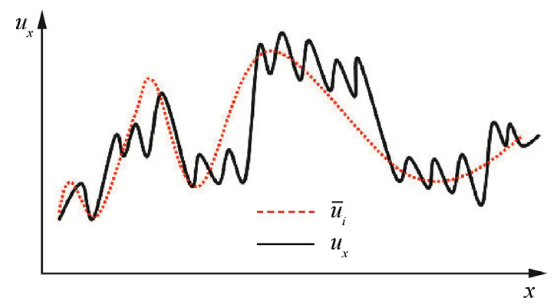
\includegraphics[width=1\textwidth]{filtered_velocity.png} % Replace with your image filename
    \caption{Velocity and filtered velocity \cite{zhiyinLargeeddySimulationPresent2015}} % Caption for the figure
    \label{filtered_velocity} % Label for referencing
  \end{figure}
\end{frame}

%------------------------------------------2
\begin{frame}
  \frametitle{Filtered Equations}
 \begin{equation}
  \frac{\partial \overline{u}_j}{\partial x_j}=0
 \end{equation}

  \begin{equation}
    \rho \left( \frac{\partial \overline{u}_i}{\partial t} + 
    \frac{\partial \overline{u}_i \overline{u}_j}{\partial x_j} \right)= 
     \rho f_i -\frac{\partial \overline{u}_i \overline{u}_j}{\partial x_j} 
     + \frac{\partial (2 \mu \overline{S}_{ij})}{\partial x_j} 
     + \frac{\partial \tau_{ij, \text{SGS}}}{\partial x_j}
  \end{equation}

  
  \begin{equation}
    \rho \left( \frac{\partial \overline{h}}{\partial t} +
     \frac{\partial \overline{h} \overline{u}_j}{\partial x_j} \right) 
     =  \frac{D \overline{p}}{D t} + \rho f_j \overline{u}_j -
      \frac{\partial \overline{q}_j}{\partial x_j} + \dot{q} +
      \frac{\partial H_j}{\partial x_j}
  \end{equation}
where 
\begin{equation}
  \tau_{ij, \text{SGS}}=-\rho (\overline{u_i u_j}-\overline{u}_i \overline{u}_j)
\end{equation}
\begin{equation}
  H_j=-\rho((\overline{h u_j}-\overline{h} \overline{u}_j))
\end{equation}

\end{frame}

%------------------------------------------2
\begin{frame}
  \frametitle{Modeling the SGS terms}
Both $\tau_{ij, \text{SGS}}$ and $H_j$ require modeling.\\
Eddy viscosity is modeled using Boussinesq hypothesis to calculate eddy viscosity \cite{zouLARGEEDDYSIMULATION2006}:
\begin{equation}
  \tau_{ij,\text{SGS}} - \frac{1}{3}\delta_{ij}\tau_{kk,SGS} =  2\rho v_T \overline{S}_{ij}
\end{equation}
The SGS heat flux is modeled with gradient-diffusion model\cite{zouLARGEEDDYSIMULATION2006}:
\begin{equation}
  H_j = \frac{\mu_T}{\text{Pr}_T} \frac{\partial \overline{h}}{\partial x_j}
\end{equation}
\end{frame}



\begin{frame}
  \bibliographystyle{plain}
  \bibliography{MyLibrary} 
  
\end{frame}


\end{document}
